\documentclass{standalone}
\usepackage{tikz}
\usepackage{ctex,siunitx}
\setCJKmainfont{Noto Serif CJK SC}
\usepackage{tkz-euclide}
\usepackage{amsmath}
\usetikzlibrary{patterns, calc,3d}
\usetikzlibrary {decorations.pathmorphing,decorations.pathreplacing,decorations.shapes}
\tikzset{label style/.append style={font=\small}}
\begin{document}
\small
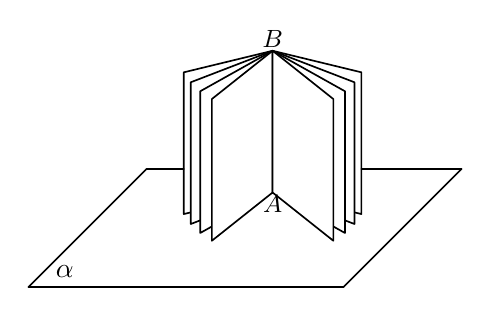
\begin{tikzpicture}[>=latex,scale=1.0,inner sep=1pt]
  \tkzDefPoints{0/0/A',4/0/B',5.5/1.5/C',1.5/1.5/D',3.1/1.2/A,3.1/3/B}
  \foreach \x[count=\i] in{200,210,220,230}
  {
    \tkzDefShiftPoint[A]({1.2*cos(\x)},{0.8*sin(\x)}){M\i}
  }
  \foreach \x[count=\i from 5] in{-20,-30,-40,-50}
  {
    \tkzDefShiftPoint[A]({1.2*cos(\x)},{0.8*sin(\x)}){M\i}
  }
  \tkzDefPointsBy[translation=from A to B](M1,M2,M3,M4,M5,M6,M7,M8){N1,N2,N3,N4,N5,N6,N7,N8}
  \tkzInterLL(C',D')(M1,N1)\tkzGetPoint{P}
  \tkzInterLL(C',D')(M5,N5)\tkzGetPoint{Q}
  \foreach \x in {1,...,8}
  {\tkzDrawPolygon[semithick,fill=white](B,N\x,M\x,A)}
  \tkzDrawSegments[semithick](A,B A',B' B',C' A',D' C',Q D',P)
  \tkzLabelPoints[above](B)
  \tkzLabelPoints[below](A)
  \tkzLabelAngle[pos=0.5](B',A',D'){$\alpha$}
\end{tikzpicture}
\end{document}